\chapter{Analyse van de resultaten}\label{sec:analyse}
In dit hoofdstuk worden de observaties in meer detail besproken. Voor elke observatie zal er geprobeerd worden een verklaren te vinden of een hypothese voor te stellen. 

Eerst zal de kalibratie aan bod komen, vervolgens de beschikbaarheids- en tenslotte de consistentietesten. Bij elke test zullen eerst de verschillende systemen besproken worden om vervolgens een vergelijking te maken. 

\section{Kalibratie}
Over de kalibratie testen valt in het algemeen niet veel af te leiden, de verschillende systemen hebben niet hetzelfde aantal instanties, zo heeft Pgpool-II slechts 3 instanties t.o.v. 6 voor MongoDB. 

Enkel op de stijgende variatie van de vertragingen in MongoDB zal dieper ingegaan worden. Bij het toenemen van het aantal gelijktijdige gebruikers neemt niet enkel de gemiddelde vertraging toe, maar ook de standaard deviatie groeit significant. Sommige bewerkingen verlopen snel, andere bewerkingen staan zeer lang in de wachtrij. De reden hiervoor is een lezers/schrijvers locking systeem op de gehele database\cite{mongodb-concurrency}. Hierdoor zorgt een leesactie voor de blokkering van alle schrijfactie op de database en vice versa. Naar mate er meer gebruikers zijn, kunnen er meer opeenvolgende schrijfoperaties zijn, dit zal de leesacties langer blokkeren. Maar indien alle gebruikers samen lezen, kan dit parallel gebeuren, een grotere variatie in de vertraging treedt hierdoor op. \\
Het gevolg van deze werkwijze is dat indien veel gebruikers actief zijn, de duur van een bewerking moeilijk te voorspellen is. Voor de resultaten van de benchmarking tool is het best om zo weinig mogelijk variatie binnen een testrun te hebben, vandaar is er gekozen voor weinig gelijktijdige gebruikers.

\section{Beschikbaarheidstest}
Bij de beschikbaarheidstesten blijkt er uit de resultaten dat de verschillende systemen een andere aanpak hebben genomen. Voor elk systeem zullen de drie testen in detail besproken worden, daarna zal een vergelijking tussen de drie systemen besproken worden. 

\paragraph{HBase} Bij HBase heeft een bepaalde HRegionServer de verantwoordelijkheid over een Regio voor een bepaalde tijd. Dit is een sessie dit door HMaster uitgedeeld wordt en bijgehouden wordt in Zookeeper. Deze sessie kan vroegtijdig beëindigd worden door de HRegionServer of er moet gewacht worden tot deze verlopen is, enkel op die momenten kan er een nieuwe HRegionServer aangeduid worden. Dit zorgt voor een duidelijk verschil tussen een zachte stop, een harde stop of een netwerk onderbreking. 

De duur van een sessie kan geconfigureerd worden in Zookeeper en staat standaard op 180 seconden. \cite{hbase-doc}. 

\subparagraph{Zachte stop} Indien een RegionServer wordt stopgezet, nemen de queries tijdelijk meer tijd in beslag. Na het stopzetten van de RegionServer is er in bepaalde gevallen een verhoogde vertraging in beide leesoperaties (scan en lees). \\ 
Het stopzetten van een HRegionServer is enkel merkbaar als er data gelezen of geschreven wordt waarvoor deze server verantwoordelijk is. In de testen worden vele bewerkingen per seconde uitgevoerd per connectie. De kans dat de HRegionServer gecontacteerd wordt kort na het stopzetten is daarom zeer groot. \\
Zodra er een herverdeling is van de HRegions over de aanwezige HRegionservers, verdwijnt deze verhoogde vertraging. De onderbreking neemt enkele seconden in beslag. 

\subparagraph{Netwerk onderbreking} Bij een netwerk onderbreking, worden de queries tijdelijk stopgezet en falen de queries in tussentijd. Deze onderbreking duurt significant langer, tot 180 seconden, dan in het geval van een zachte stop. Dit komt doordat de regio's pas kunnen toegewezen worden na het verlopen van hun sessie.  

\subparagraph{Harde stop} Bij het stopzetten van een instantie op de harde manier, zijn er twee reacties: de eerste is vergelijkbaar met deze van een netwerk onderbreking. De andere laat pas opnieuw queries toe na het herstellen van het netwerk verkeer. In een manuele test bleek dit opgelost te zijn na het verbreken van de connectie en het opnieuw verbinden, maar de oorzaak waarom deze permanente onderbreking af en toe ontstaat, is niet gevonden. 

\subparagraph{Herstel van de instantie} Het herstel van de server zal automatisch op een asynchrone manier gebeuren. Er valt te configureren hoeveel netwerkverkeer er maximaal per seconde zal worden gebruikt voor de synchronisatie. Het herstel is niet merkbaar voor de gebruiker op de vertraging van de bewerkingen. 

\paragraph{MongoDB} Bij MongoDB is er tussen de leden van een Replicaset een heartbeat protocol. Indien er gedurende 10 seconden geen antwoord op een een heartbeat komt, wordt een server als offline bestempeld. De server die als laatste contact met de primary heeft gehad zal zijn rol overnemen indien de primary onbereikbaar wordt\cite{mongodb-manual}. Dit heeft zijn invloed op de verschillende manieren om een server stop te stopzetten. 

\subparagraph{Zachte stop en harde stop} Bij een zachte of harde stop is er een kans van 1 op 3 dat het uitvallen van een instantie zichtbaar is, dit is te verklaren doordat een replicaset bestaat uit drie server in onze configuratie. In de standaard modus wordt er enkel gelezen naar en geschreven van de primary, indien deze onbereikbaar wordt is er een onderbreking. Na het kiezen van een nieuwer primary is er geen verschil in vertraging per soort query ten opzichte van ervoor. Er zijn 2 hypothesen waarom een harde stop op dezelfde manier reageert: bij een harde stop wordt de sessie nog altijd vrijgegeven, of er zijn verkiezingen voor een nieuwe primary voordat de sessie van de oude primary is afgelopen. Deze hypothesen zijn niet getest of verder onderzocht. 

\subparagraph{Netwerk onderbreking} Bij een netwerk onderbreking zou het te verwachten zijn dat na maximaal 10 seconde de primary zou veranderen. Onder de aangelegde belasting blijkt dat de database heel de tijd onbeschikbaar tot de primary opnieuw bereikbaar is via het netwerk. Bij het manueel testen blijkt dat er dezelfde foutmelding gegeven wordt als bij het stoppen van de database, maar dat de data onbeschikbaar is. Het volstaat om de verbindingen af te sluiten en opnieuw aan te maken om het probleem op te lossen. Er is geen reden gevonden voor dit gedrag. 

\subparagraph{Herstel van de instantie} Het herstel van de server zal automatisch op een asynchrone manier gebeuren. Dit is niet merkbaar voor de gebruikers en de server zal als secondary ingezet worden. 

\paragraph{Pgpool-II} Bij Pgpool-II wordt de status van de PostgreSQL instanties getest wanneer er een gebruiker actief is.  Bij het uitvallen van een instantie en opnieuw opstarten terwijl er geen gebruiker verbonden is met Pgpool-II, zal dit niet opgemerkt worden. Daarnaast zijn er verschillende reacties op de geteste scenario's. 

Een vereiste bij het herstellen van een instantie is dat er op dat moment geen enkele verbinding met de router instantie is. 

\subparagraph{Zachte stop} Bij een zachte stop van een data instantie worden alle verbinden van de gebruikers met Pgpool-II onmiddellijk verbroken. Nadien kan er terug verbonden worden met Pgpool-II. In deze omgeving gaan nadien de verschillende schrijfoperaties sneller omdat deze niet meer gerepliceerd moeten worden. Een hypothese is dat bij een grote hoeveelheid data instanties dit effect kleiner zal worden.  

\subparagraph{Harde stop} Een harde stop reageert hetzelfde als een zachte stop. Dit omdat ook hier de connecties onmiddellijk verbroken zijn. Het besturingssysteem van de data instantie zal antwoorden dat er geen service op de poort aan het luisteren is en Pgpool-II detecteert de fout. 

\subparagraph{Netwerk onderbreking} Bij een netwerk onderbreking is er een ander gedrag, de queries wachten op een antwoord maar krijgen dit niet. Hierdoor worden alle bewerkingen geblokkeerd tot een antwoord of de time-out van de connecties naar de dataserver die standaard 30 seconde is. In dit geval is er een time-out en gebeurt de interne overschakeling. Hierbij worden alle connecties van de gebruikers verbroken en de onbereikbare server niet meer gebruikt. Daarna kan de gebruiker opnieuw verbinden met Pgpool-II en queries uitvoeren. 

\subparagraph{Vermindering van schrijfvertraging} De reden tot de vermindering van de schrijfvertraging is te verklaren door de wijze waarop Pgpool-II de schrijfbewerkingen uitvoert. Deze zullen eerst op de master uitgevoerd worden en vervolgens op de verschillende slaves. Bij het wegvallen van een instantie is er in de testopstelling nog maar een enkele dataserver over, hierdoor duurt een schrijfactie maar half zo lang. De leesacties duren ongeveer even lang aangezien er nog steeds gelezen wordt van een dataserver. 

\subparagraph{Herstel van de instantie} Bij het opnieuw inschakelen van een instantie dient in Pgpool-II het herstel handmatig opgestart te worden. De data zal van de master naar de instantie gesynchroniseerd worden. In het geval van een grote achterstand zal dit merkbaar zijn omdat dit proces aan maximale snelheid wordt uitgevoerd; een grote belasting op de CPU, harde schijf en het netwerk kunnen dus voorkomen voor het lezen, comprimeren en versturen van de data. Om het herstel te voltooien moeten alle connecties naar Pgpool-II op een gegeven moment gesloten worden. In de testen die werden uitgevoerd was er continue dataverkeer en werden er nieuwe databasebewerkingen naar Pgpool-II gestuurd, hierdoor slaagde het herstel niet. 

\paragraph{Samenvatting} Zowel HBase als MongoDB volgen de status de hele tijd op. Bij HBase is dit de verantwoordelijkheid van Zookeeper waarbij onder andere de sessieduur geconfigureerd worden. Bij MongoDB wordt dit afgehandeld door de verschillende services zelf en is er geen configuratiemogelijkheid. Pgpool-II gebruikt een princiepe door enkel de instanties te controleren op het moment dat er een verbinding is. \\
Daarnaast ondersteunt Pgpool-II ook niet de automatische herstel en komt de handmatige herstel niet tot voltooiing onder constant gebruik, hiervoor zijn beide andere systemen automatischer. Een overzicht van het gedrag bij het stoppen en starten van een instantie , bevinden zich in tabel \ref{table:beschikbaarheid-stop-resultaat} en \ref{table:beschikbaarheid-herstel-resultaat}. \\
Doordat er een matige belasting is van de verschillende systemen is het effect tijdens het onbeschikbaar zijn van de service beperkt naar de duur van de bewerkingen als ook het herstel. De verschillende werkende servers kunnen de extra belasting opvangen, bij een hoge belasting zou het kunnen zijn dat er wel een effect is. 

\begin{table}[htbp]
  \centering
    \begin{tabular}{l | lll}
          & Zachte stop & Harde stop & Netwerk stop \\
    \hline
    \multirow{2}{*}{HBase} & Enkele seconden & Tiental seconden & Tiental seconden \\
    & & of onbeperkt&  \\
    \multirow{2}{*}{MongoDB} & 1/3 van de gevallen, & 1/3 van de gevallen, & Enkele seconden tot \\
    & enkele seconden & enkele seconden & Onbeperkt\\
    Pgpool-II & Enkele seconden & Enkele seconden & 30 seconden \\
    \end{tabular}%
    \caption{Beschikbaarheid: Overzicht van de reacties bij het stoppen van een instantie }
  \label{table:beschikbaarheid-stop-resultaat}%
\end{table}

\begin{table}[htbp]
  \centering
    \begin{tabular}{l|l}
          & Automatisch herstel \\
    \hline
    HBase & Ja \\
    MongoDB & Ja \\
    Pgpool-II & Nee \\
    \end{tabular}%
      \caption{Beschikbaarheid: Overzicht van de ondersteuning van automatisch herstel}
  \label{table:beschikbaarheid-herstel-resultaat}%
\end{table}%

\paragraph{Implicatie van de resultaten voor een gebruiker} De drie systemen kunnen opgesplitst worden in twee groepen. Indien de ontwikkelaar van een softwaresysteem een systeem wilt dat keer op keer hetzelfde reageert op het onbeschikbaar worden van een server, dan kiest hij het best voor Pgpool-II. Het nadeel van deze keuze is dat voor het herstel tijdelijk de database connecties moet verbroken worden. Ook Pgpool node kan een limiterende factor worden naar de schaling, maar met de parallelle mode van Pgpool-II kan dit overwonnen worden. \\

Wil men daartegen een systeem met automatisch herstel, dan kan men kiezen voor HBase of MongoDB. Als de ontwikkelaar het gedrag bij faling in detail zelf wilt configureren, heeft HBase vele configuratie mogelijkheden. MongoDB is hierin meer beperkt maar biedt een systeem aan dat standaard sneller herstelt. Voor beide systemen kan het soms nodig zijn om een connectie te verbreken en een nieuwe connectie op te zetten als een service onbeschikbaar wordt. 

\section{Consistentietest}
\paragraph{HBase} HBase garandeert strikte consistentie op een enkel record en hoe deze garantie tot uitvoering wordt gebracht, is zichtbaar in figuren \ref{fig:consistentie-hbase-tijdschaal-lezer-1} en \ref{fig:consistentie-hbase-R1}. Een leesbewerking wordt namelijk op wacht gezet tot de schrijfbewerking voltooid is. In de eerste figuur wacht de leesbewerking met afronden van zijn bewerking tot de schrijfbewerking is voltooid. Indien een leesbewerking vroeger gedaan heeft, moet deze een tweede poging ondernemen omdat deze de eerste keer oude data heeft gelezen. In de tweede figuur heeft de lijn van het stoppen met lezen van de correcte waarde continue een hogere waarde dan het voltooien van de schrijfbewerking. \\
Dit gedrag is te verklaren doordat HBase gebruik maakt van lezer/schrijvers locking, hierdoor moet een leesactie wachten tot een schrijfactie de lock terug vrij geeft. In figuur \ref{fig:consistency-hbase-uitleg} wordt het lees- en schrijfmodel in detail uitgelegd aan de hand van de beschrijving van Lars Hofhansl\cite{hbase-acid}. De combinatie van een enkele HRegionServer voor een record en het gebruiken van locks, zorgt ervoor dat atomaire acties op een enkele record succesvol afgedwongen kunnen worden.     

Uit de testresultaten blijkt dat indien de leesbewerking te snel verstuurd wordt, er nog geen blokkering van de bewerking zal plaats vinden. Het percentage van de queries dat de nieuwe data zal lezen, bevindt zich in figuur \ref{fig:consistentie-hbase-correct}.


\begin{figure}[!htf]

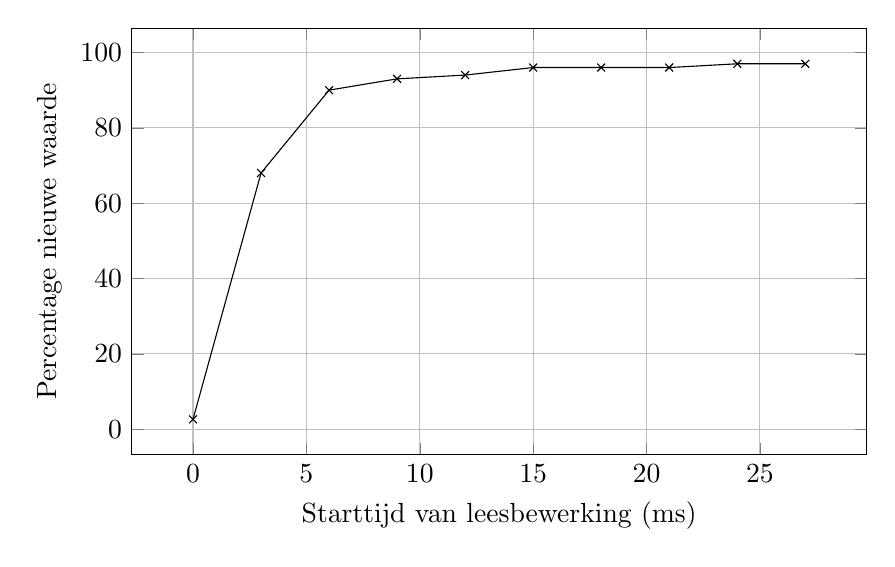
\begin{tikzpicture}
	
	\begin{axis}[
		xlabel={Starttijd van leesbewerking (ms)},
		ylabel={Percentage nieuwe waarde},
		domain = 0:1,
		grid = major,
		height=7cm,
		width=.9\textwidth
	]
	

	\addplot[color=black,mark=x]
	        plot coordinates {
	       		(0, 2.6)
				(3, 68)
				(6,90)
				(9,93)
				(12,94)
				(15,96)
				(18,96)
				(21,96)
				(24,97)
				(27,97)
	        };

	\end{axis}
\end{tikzpicture}
\caption{Consistentie: Percentage van de queries dat op een gegeven tijdstip de juiste data leest voor HBase. Het gemiddelde verschil tussen het starten en stoppen van het lezen op een willekeurig record is ongeveer 6ms, in het geval van hetzelfde record kan dit langer duren door het wachten op de lock. }
\label{fig:consistentie-hbase-correct}
\end{figure}


\begin{figure}[tb!]
	\begin{minipage}{0.5\textwidth} 
	\textbf{Schrijven}
	\begin{enumerate}
	\item Lock de rij(en), om te beschermen tegen gelijktijdige lees- en schrijfacties. 
	\item Haal het huidige schrijfnummer op
	\item Voeg aanpassingen toe aan WAL (Write Ahead Log)
	\item Pas aanpassing toe op de Memstore (cache geheugen)
	\item Commit de transactie, m.a.w. zet het leespunt op het nieuwe schrijfnummer
	\item Unlock de rijen
	\end{enumerate}
	\end{minipage} \hfill
	\begin{minipage}{0.3\textwidth} 
	\textbf{Lezen}
	\begin{enumerate}
	\item Open de lezer
	\item Ga naar het huidige leespunt
	\item Filter al de Key-Value paren met schrijfnummer > leespunt
	\item Sluit de lezer
	\end{enumerate}
	\end{minipage}
	\caption{HBase: Het vereenvoudigde lees- en schrijfmodel voor strikte consistentie in HBase naar Lars Hofhansl\cite{hbase-acid}}\label{fig:consistency-hbase-uitleg}
\end{figure}

\paragraph{MongoDB} MongoDB biedt strikte consistentie aan als er van de primary gelezen wordt maar er zijn ook andere schrijf- en leesmethodes. Een verschil met HBase is dat het bij alle mogelijke lees- en schrijfmethodes mogelijk is om de nieuwe data al te lezen vooraleer de schrijfbewerking beëindigd is. Een schrijfbewerking wacht op de server nog na het schrijven en vrijgeven van zijn schrijf lock. Een verklaring is hiervoor niet gevonden.

Uit figuren \ref{fig:consistentie-mongodb-primary}, \ref{fig:consistentie-mongodb-primarypreferred}, \ref{fig:consistentie-mongodb-secondary}, \ref{fig:consistentie-mongodb-secondarypreferred} en \ref{fig:consistentie-mongodb-nearest} kan een analyse gemaakt worden hoeveel kans er is dat een leesbewerking de nieuwe data al zal lezen. Voor lezer 1 tot 5, dit zijn tijdstippen 0, 2, 4, 6 en 8 ms, is een kans berekend ten opzichte van het starttijdstip. Een grafische voorstelling voor de vier leesconfiguratie bevindt zich in figuur \ref{fig:consistentie-mongodb-correct}. 

Uit figuren \ref{fig:consistentie-mongodb-verschillende-schrijfacties} blijkt dat er geen significant verschil is tussen de leesacties onder verschillende schrijfgaranties, indien men de starttijdstippen vergelijkt. De schrijfconfiguraties geven geen garanties tijdens het uitvoeren maar geven verschillende garanties als de schrijfactie voltooid is.

Uit tabel \ref{table:consistentie-mongodb-inconsistency} blijkt dat het in MongoDB niet gegarandeerd is dat als een lezer de nieuwe waarde leest, al de andere lezers dit ook zullen doen. In het voorbeeld was het schrijven nog niet voltooid maar toch las een bepaalde lezer de nieuwe data al. Een leesbewerking die later gestart is, leest de oude waarde nog. Dit kan verklaard worden doordat het verschillende servers zijn waarop gelezen wordt. Het waren verschillende lezers, maar de MongoDB driver controleert periodiek welke server het dichtste bij is en kan een nieuwe server kiezen als nearest. Een hypothese is dat de leesserver kan veranderen tussen twee bewerkingen gebeuren en hierdoor na het lezen van de nieuwe waarde op bijvoorbeeld de primary, de tweede keer nog de oude data op een secondary gelezen wordt. Om deze reden wordt er verondersteld dat er geen garantie is op monotone consistentie als men niet lees van de primary. 

In de testomgeving is er een uniforme netwerkvertraging tussen alle servers. De theoretische kans dat een dichtstbijzijnde server een primary is, is 1 op 3, voor een secondary is dit 2 op 3. Het gedrag in de praktijk voor consistentie heeft minder dan 5\% afwijking van dit theoretisch model. De testresultaten van nearest kunnen dus ook afgeleid worden in de toekomst uit de resultaten van primary en secondary. 

Tenslotte hebben primary en primary-preferred in deze testen geen significante verschillen. Dit komt omdat de primary heel de tijd beschikbaar is en er niet overgeschakeld moet worden naar de secondary. 

\begin{table}
\centering
\begin{tabular}{l | l l l l}
Lezer & Start lezen (ms) & Stop lezen (ms) & Gelezen waarde & Correct? \\
\hline
\multirow{2}{*}{1} & 2,200 & 3,213 & 12553\textbf{3}813315 & Nee\\
 & 13,426 & 14,279 & 12553\textbf{4}813315 & Ja \\
 \multirow{2}{*}{3} & 17,458 & 18,834 & 12553\textbf{3}813315 & Nee\\
 & 29,063 & 29,897 & 12553\textbf{3}813315& Ja \\
\end{tabular}
\caption{Consistentie: Ruwe data van MongoDB test waarbij inconsistente data wordt gelezen na het lezen van consistente data op verschillende lezers met het lezen via nearest en schrijven via fsync\_safe}
\label{table:consistentie-mongodb-inconsistency}
\end{table}


\begin{figure}[!htf]

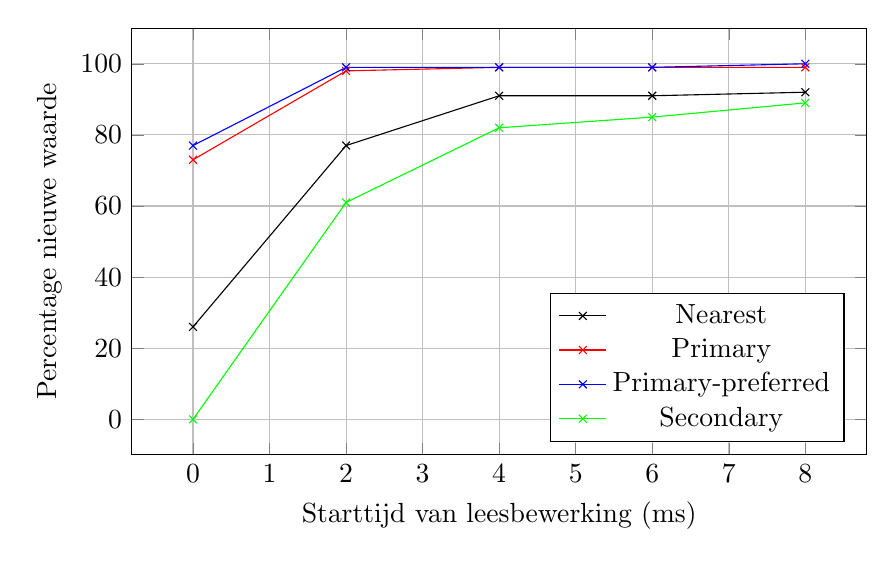
\begin{tikzpicture}
	
	\begin{axis}[
		xlabel={Starttijd van leesbewerking (ms)},
		ylabel={Percentage nieuwe waarde},
		domain = 0:1,
		grid = major,
		height=7cm,
		width=.9\textwidth,
		legend pos= south east
	]
	
	\addplot[color=black,mark=x]
	        plot coordinates {
	       		(0, 26)
				(2, 77)
				(4,91)
				(6,91)
				(8,92)
	        };
	\addlegendentry{Nearest}

	\addplot[color=red,mark=x]
	        plot coordinates {
	       		(0, 73)
				(2, 98)
				(4,99)
				(6,99)
				(8,99)
	        };
	\addlegendentry{Primary}
	
	\addplot[color=blue,mark=x]
      plot coordinates {
	       		(0, 77)
				(2, 99)
				(4,99)
				(6,99)
				(8,100)
      };
	\addlegendentry{Primary-preferred}
	
	\addplot[color=green,mark=x]
   plot coordinates {
	       		(0, 0)
				(2, 61)
				(4,82)
				(6,85)
				(8,89)
   };
	\addlegendentry{Secondary}
	\end{axis}
\end{tikzpicture}
\caption{Consistentie: Percentage van de queries dat van de eerste keer juist de data leest bij 0ms, 2ms, 4ms, 6ms en 8ms voor MongoDB. De gemiddelde vertraging op een onafhankelijke leesoperatie is 1ms. }
\label{fig:consistentie-mongodb-correct}
\end{figure}


\paragraph{Samenvatting} Beide database systemen bieden strikte consistentie aan maar hebben een verschillende uitwerking hiervan: bij HBase worden de leesoperaties uitgesteld tot de volledige voltooiing van de schrijfoperatie, bij MongoDB zal de data al vroeger beschikbaar zijn. Beide systemen zijn \textit{session} consistent, \textit{read-your-own-write} en monotoon consistent, indien er bij MongoDB op een primary wordt gelezen.  

\textit{Session}, \textit{read-your-own-write}, \textit{casual} en \textit{monotonic} consistentie zijn niet gegarandeerd in MongoDB indien er niet gelezen wordt op een primaire. De MongoDB driver kan op ieder moment een andere server kiezen in deze gevallen en kan dus nog oude data lezen op een andere server.

Een hypothese is dat het falen van de primary de consistentie garanties zou beïnvloeden. Indien de laatste schrijfactie nog niet gerepliceerd is nog een secondary maar al wel gelezen is door een gebruiker, zal de data niet beschikbaar zijn op de nieuwe primary. De nieuwe data zal voor lezers dus niet meer beschikbaar zijn, er zou dus geen strikte consistentie in de primary leesconfiguratie kunnen zijn. Dit gedrag is wel niet bevestigd met testen in de praktijk. Een andere hypothese is dat HBase heeft deze situatie niet voor heeft omdat de leesbewerkingen uitgesteld worden tot na het voltooien van de schrijfacties.

\paragraph{Implicatie van de resultaten voor een gebruiker} MongoDB en HBase bieden in de standaardconfiguratie ongeveer dezelfde garanties. Indien het voor de ontwikkelaar belangrijk is dat nieuwe data zo snel mogelijk beschikbaar is of zelf de consistentie-eigenschappen wenst te kiezen, dan is MongoDB een goede keuze. Mag de data slechts beschikbaar zijn nadat de schrijfbewerking voltooid is, dan kan er voor HBase gekozen worden. Een situatie die deze laatste garantie kan afdwingen, is bijvoorbeeld een beurssysteem: het is mogelijk voor andere gebruikers om een aankoop te weten te komen vooraleer de koper zelf de bevestiging heeft gekregen. 

\section{Conclusie}
De drie systemen hebben verschillende aanpak voor beschikbaarheid en consistentie. Pgpool-II heeft door zijn centrale aanpak met behulp van de Pgpool-II node een consequent gedrag bij het onbeschikbaar worden van een dataserver. Daartegenover staat wel dat dit systeem geen automatisch herstel heeft maar manuele interventie vereist dat het volledige systeem tijdelijk onbereikbaar maakt. 

Het gedrag van MongoDB bij het onbeschikbaar worden van een instantie, is weinig configureerbaar. De resultaten zijn voorspelbaar maar het is mogelijk dat een database connectie niet automatisch correct wordt hersteld. Nieuwe data in veel gevallen al beschikbaar voor het voltooien van de schrijfbewerking. Daarnaast zijn er veel mogelijkheden om de garanties te configureren voor het lezen en schrijven van data. Indien er gelezen wordt van de primary bevestigen de testen dat er stikte consistentie is, het is wel onduidelijk welke garanties er zijn bij het falen van een primary. 

Met behulp van Zookeeper kan de reactie op het onbeschikbaar zijn van een server in HBase in geconfigureerd worden, onder andere door de duur van een sessie te veranderen. Ook hier is het mogelijk dat een database connectie niet automatisch wordt hersteld. Het systeem garandeert strikte consistentie. Een leesopdracht van een record die binnenkomt tijdens het schrijven of aanpassen van dat record, zal in de wachtrij gezet worden om de nieuwe data te lezen nadat de schrijfbewerking voltooid is. In de testen werd de nieuwe data nooit gelezen voor het voltooien van de schrijfbewerking. 